\section{Method}
\label{sec:method}

\begin{figure*}
\centering
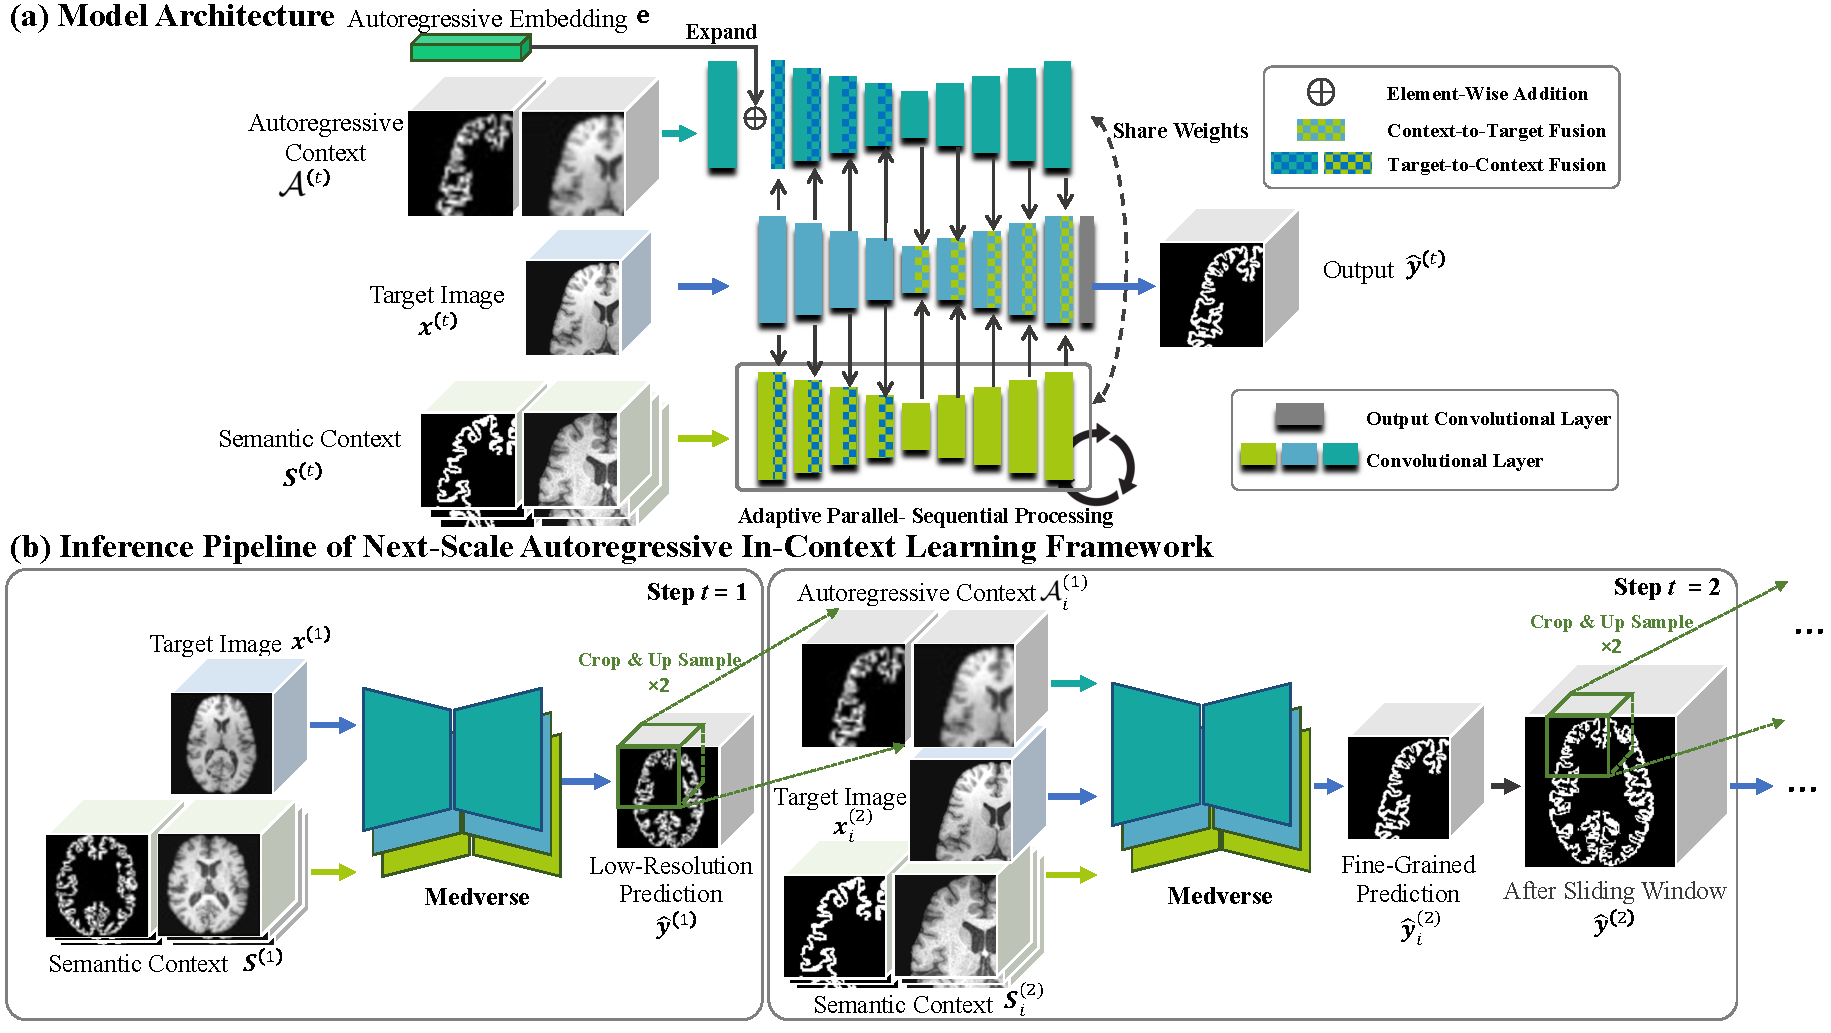
\includegraphics[width=0.85\textwidth]{main_fig.pdf}
\caption{Illustration of our model architecture and the inference pipeline of the next-scale autoregressive in-context learning framework.}
\label{fig:main_fig}
\end{figure*}

Under the ICL paradigm, Medverse achieves universality by learning task-specific guidance from context examples in the form of image-label pairs. It is capable of performing diverse tasks by leveraging the rich information embedded in these contexts.

\subsection{Next-Scale Autoregressive ICL}
Unlike conventional ICL models that utilize only context from other subjects, our NA-ICL framework provides the model with both image-label pairs from other subjects and the model's coarse predictions at lower resolutions, inspired by~\cite{tian2024visual}. This architectural design enables progressive processing from coarse to fine scales, offering benefits including the integration of multi-scale anatomical information, improved consistency across patches, and high-fidelity outputs.

\vspace{0.4em}
\noindent\textbf{Network Architecture.}
As shown in Figure~\ref{fig:main_fig} (a), the proposed model comprises three 3D U-Net branches that, from top to bottom, process the autoregressive context, the target image, and the semantic context. The target image branch interacts with both context branches through fusion modules to facilitate the context-target feature interaction.


The autoregressive context comprises the target image and its associated prediction from a lower-resolution step, and is treated as a specialized type of context. The semantic context consists of a set of image-label pairs drawn from other subjects, providing conventional semantic guidance for the task. To promote parameter efficiency and shared contextual understanding, the autoregressive context branch shares weights with the semantic context branch. To differentiate the features from the autoregressive context, we introduce a learnable autoregressive embedding $\bm{e} \in \mathbb{R}^{C}$, which is added to the output of the first layer of the autoregressive context branch as follows:
\begin{equation}
    \bm{f}^{'}_{1, \text{AR}} = \bm{f}_{1, \text{AR}} + \operatorname{Expand}(\bm{e}),
\end{equation}
where $\bm{f}_{1, \text{AR}} \in \mathbb{R}^{C \times H \times W \times D}$ denotes the feature map from the first layer and $\operatorname{Expand}(\cdot)$ expands the embedding across spatial dimensions.

Let the semantic context be defined as $S^{(t)}$, which contains a number of image-label examples. $t$ refers to the corresponding autoregressive step, which will be detailed later. Given the target image $\bm{x}^{(t)}$ and the autoregressive context from the previous step, $\mathcal{A}^{(t-1)} = (\bm{x}^{(t-1)}, \hat{\bm{y}}^{(t-1)})$, the model prediction at step $t$ is computed as
\begin{equation}
\hat{\bm{y}}^{(t)} = F(\bm{x}^{(t)},\, S^{(t)},\, \mathcal{A}^{(t-1)}),
\end{equation}
where $F(\cdot)$ denotes the prediction function of Medverse. To efficiently handle a large number of semantic context examples, we incorporate the adaptive parallel-sequential context processing module introduced in~\cite{hu2025building}, which enables scalable context processing with minimal memory requirements.

\vspace{0.4em}
\noindent\textbf{Autoregressive Inference Pipeline.}  
Given an input volume of size $(H,W,D)$, the number of autoregressive steps is
\begin{equation}
T=\bigl\lceil\log_{2}\bigl(\frac{\max\{H,W,D\}}{I}\bigr)\bigr\rceil+1,
\end{equation}
where $I\times I\times I$ denotes the model’s input patch size.
For step $t\in\{1,\dots,T\}$, we downsample the input images to
\begin{equation}
\bigl(H^{(t)},W^{(t)},D^{(t)}\bigr)=\bigl\lceil \frac{H}{2^{\,T-t}}\bigr\rceil,\;
\bigl\lceil \frac{W}{2^{\,T-t}}\bigr\rceil,\;
\bigl\lceil \frac{D}{2^{\,T-t}}\bigr\rceil,
\end{equation}
so that the resolution is doubled from level $t$ to $t+1$. We assume that the context and target images share the same spatial dimensions and undergo identical resizing operations. After the final step $t=T$, the model outputs a prediction at the original image resolution.

Figure~\ref{fig:main_fig} (b) illustrates the autoregressive inference pipeline. At step $t=1$, the model predicts $\hat{\bm{y}}^{(1)} = F(\bm{x}^{(1)},\, S^{(1)},\,\mathcal{A}^{(0)})$ on the low-resolution input image, capturing global anatomical context, with $\mathcal{A}^{(0)}$ initialized as an empty set. The autoregressive context $\mathcal{A}^{(1)} = (\bm{x}^{(1)}, \hat{\bm{y}}^{(1)})$ is then passed to step $t=2$. At $t=2$, the increased resolution requires the target image $\bm{x}^{(2)}$ to be split into $I \times I \times I$ patches, which are processed with a sliding window to capture finer anatomical detail. The prediction for each patch $\bm{x}^{(2)}_i$ is then given by $\hat{\bm{y}}^{(2)}_i = F(\bm{x}^{(2)}_i,\, S^{(2)}_i,\, \mathcal{A}^{(1)}_i)$. $S^{(2)}_i$ denotes the semantic context cropped at the same spatial location as $\bm{x}^{(2)}_i$ to ensure patch-wise alignment. To propagate global information from coarser scales, the corresponding region in $\mathcal{A}^{(1)}$ of size $\frac{I}{2} \times \frac{I}{2} \times \frac{I}{2}$ is extracted, upsampled to $I \times I \times I$, and used as $\mathcal{A}^{(1)}_i$. The same procedure is repeated for $t \ge 2$, with the number of sliding windows increasing as the resolution increases. A step-by-step pseudocode is provided in the supplementary material.

\begin{figure*}
\centering
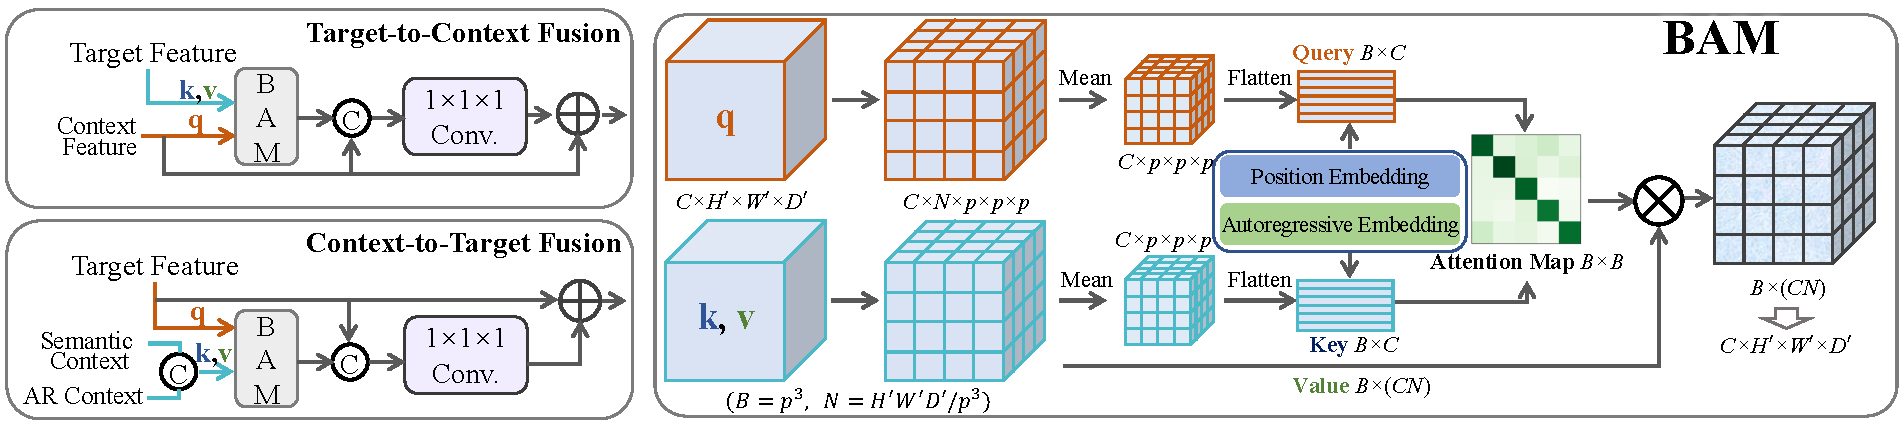
\includegraphics[width=0.99\textwidth]{cross_attention.pdf}
\caption{Illustration of fusion modules and the blockwise cross-attention module.}
\label{fig:bam}
\end{figure*}

\subsection{Context-Target Fusion Module}  
Feature interaction between different branches in the network is achieved through fusion modules, enabling the target branch to effectively incorporate contextual information. As shown in Figure~\ref{fig:main_fig} (a), we perform target-to-context fusion within the encoder, where features from the target branch are passed to the context branch, and context-to-target fusion within the decoder, where features from the context branch are passed back to the target branch. The use of adaptive parallel-sequential context processing necessitates this order of interaction.

The details of the fusion module are illustrated in Figure~\ref{fig:bam}.
The target-to-context module employs the context feature map as the query, with the target feature map serving as the source of keys and values.
BAM transfers target information to the context, after which the output is concatenated with the original context, compressed by a $1\times1\times1$ convolution, and added back through a residual shortcut to produce a target-aware context representation.

The context-to-target fusion module concatenates semantic and autoregressive context features, using the combined representation as the source of keys and values, with the target features serving as the query. BAM injects both semantic and autoregressive contextual guidance into the target representation. The resulting features are then similarly passed through concatenation, convolution, and a residual shortcut to produce a context-aware target representation.


% _____________________________________________________________________________________________


\vspace{0.4em}\noindent\textbf{Blockwise Cross-Attention Module.}  
Since there is not necessarily strict spatial alignment between the context and target objects, long-range interactions are crucial for effective feature fusion. We propose BAM, which enables efficient long-range feature aggregation with spatial sparsity.

We denote the query feature map by
$\bm{X}_{q}\!\in\!\mathbb{R}^{C\times H'\times W'\times D'}$, and
the key–value map by
$\bm{X}_{kv}\!\in\!\mathbb{R}^{C\times H'\times W'\times D'}$.
The volume is partitioned into
$p\times p\times p$ non-overlapping blocks,
so that each block covers
$h=\frac{H'}{p}$,
$w=\frac{W'}{p}$,
and
$d=\frac{D'}{p}$ voxels.
Let $N = hwd$ denote the number of voxels per block.
After partitioning, we obtain the blockwise features
$\bm{X}_{q}^{\text{Blockwise}},\, \bm{X}_{kv}^{\text{Blockwise}} \in \mathbb{R}^{C \times N \times p \times p \times p}$.
The query and key representations for each block are then computed by mean pooling over the $N$ voxels within the block:
\begin{align}
\bm{Q}' &= \frac{1}{N} \sum_{n=1}^{N} \bm{X}_{q}^{\text{Blockwise}}[:, n, :, :,:] \in \mathbb{R}^{C\times p\times p\times p}, \\
\bm{K}' &= \frac{1}{N} \sum_{n=1}^{N} \bm{X}_{kv}^{\text{Blockwise}}[:, n, :, :, :] \in \mathbb{R}^{C\times p\times p\times p}.
\end{align}


To match the input format required by the attention mechanism, we transpose and reshape $\bm{Q}'$ and $\bm{K}'$ to obtain
$\bm{Q}, \bm{K} \in \mathbb{R}^{B \times C}$, where $B = p^{3}$ denotes the total number of blocks.
Then, the queries and keys are linearly projected into a $m$-dimensional space via
learnable matrices $\bm{W}_Q, \bm{W}_K \in \mathbb{R}^{C \times m}$.
To incorporate spatial priors, we add a 3D sine–cosine positional embedding
$\bm{P} \in \mathbb{R}^{B \times m}$ to both branches.
In addition, for blocks originating from the autoregressive context,
we further add a learnable autoregressive embedding
$\bm{R} \in \mathbb{R}^{m}$,
which acts as a marker for features from the autoregressive branch and is broadcast across all blocks to shape $B \times m$.
The resulting transformed features are given by
\begin{align}
\widehat{\bm{Q}} &= \bm{Q} \bm{W}_Q + \bm{P} + \bm{1}_{\text{AR}} \cdot \bm{R}, \\
\widehat{\bm{K}} &= \bm{K} \bm{W}_K + \bm{P} + \bm{1}_{\text{AR}} \cdot \bm{R},
\end{align}
where $\bm{1}_{\text{AR}}$ is an indicator that equals 1 if the block comes
from the autoregressive context and 0 otherwise. The block-level attention weights are as follows:
\begin{align}
\bm{A}=
\operatorname{Softmax}\!\Bigl(
\frac{\widehat{\bm{Q}}\widehat{\bm{K}}^{\!\top}}{\sqrt{m}}
\Bigr)\in\mathbb{R}^{B\times B}.
\end{align}

To preserve spatial granularity, the value features are obtained directly from the unpooled input as $\bm{V}' = \bm{X}_{kv}^{\text{Blockwise}} \in \mathbb{R}^{C \times N \times p \times p \times p}$. They are then transposed and reshaped to match the input format for attention dot-product computation, yielding $\bm{V} \in \mathbb{R}^{B \times (C N)}$. The value matrix $\bm{V}$ is multiplied by the attention weights to obtain
\[
\bar{\bm{Y}} = \bm{A}\,\bm{V}
      \in \mathbb{R}^{B \times (C N)}.
\]
The result is then reshaped back to the original spatial layout,
producing the final BAM output:
\[
\widehat{\bm{Y}}
  = \operatorname{Reshape}\bigl(\bar{\bm{Y}}\bigr)
  \in \mathbb{R}^{C \times H' \times W'\times D'}.
\]


The computational complexity is thereby reduced to $\mathcal{O}(B^{2})$, in contrast to the original $\mathcal{O}\!\bigl((H'W'D')^{2}\bigr)$, while still preserving long-range interactions and retaining fine-grained value information. $B = p^3$ is a user-defined constant that remains fixed across U-Net stages, further ensuring stable computational cost. Compared to the direct concatenation-based fusion used in~\cite{butoi2023universeg,czolbe2023neuralizer, hu2025building}, this cross-attention fusion approach is better suited for handling spatial misalignment between the context and target objects.

\subsection{Loss Function}
For fair comparison, we adopt the same loss functions as those proposed in~\cite{hu2025building}. Specifically, a modified $\mathcal{L}_{\text{smooth}-L_{1}}$ loss is used for segmentation tasks, while for image enhancement and transformation tasks, the $\mathcal{L}_{\text{smooth}-L_{1}}$ loss is applied to both image intensity and intensity differences.


